%%%%%%%%%%%%%%%%%%%%%%%%%%%%%%%%%%%%%%%%%%%%%%%%%%%%%%%%%%%%%%%%%%%%%%%%%%%%%%%%
% AMS Beamer series / Bologna FC / Template
% Andrea Omicini
% Alma Mater Studiorum - Università di Bologna
% mailto:andrea.omicini@unibo.it
%%%%%%%%%%%%%%%%%%%%%%%%%%%%%%%%%%%%%%%%%%%%%%%%%%%%%%%%%%%%%%%%%%%%%%%%%%%%%%%%
%\documentclass[handout]{beamer}\mode<handout>{\usetheme{default}}
%
\documentclass[presentation, 9pt]{beamer}\mode<presentation>{\usetheme{AMSBolognaFC}}
%\documentclass[handout]{beamer}\mode<handout>{\usetheme{AMSBolognaFC}}
%%%%%%%%%%%%%%%%%%%%%%%%%%%%%%%%%%%%%%%%%%%%%%%%%%%%%%%%%%%%%%%%%%%%%%%%%%%%%%%%
\usepackage[T1]{fontenc}
\usepackage[minted,most]{tcolorbox}
\usepackage{wasysym}
\usepackage{amsmath,blkarray}
\usepackage{centernot}
\usepackage{fontawesome}
\usepackage{fancyvrb}
\usepackage{lmodern}
\usepackage[ddmmyyyy]{datetime}
\newcounter{totalcontinuationcount}
\makeatletter
\setbeamertemplate{frametitle continuation}{%
    \setcounter{totalcontinuationcount}{\beamer@endpageofframe}%
    \addtocounter{totalcontinuationcount}{1}%
    \addtocounter{totalcontinuationcount}{-\beamer@startpageofframe}%
    \ifnum \value{totalcontinuationcount} > 1
        \textmd{(\insertcontinuationcount/\arabic{totalcontinuationcount})}%
    \fi
}
\makeatother
\setbeamertemplate{enumerate item}{\insertenumlabel.}
\renewcommand{\dateseparator}{}
%\renewcommand{\thefootnote}{\fnsymbol{footnote}}
\newcommand{\version}{1}
\usepackage[
	backend=biber,
	citestyle=authoryear-icomp,
	maxcitenames=1,
	bibstyle=alphabetic]{biblatex}

	\makeatletter

\addbibresource{biblio.bib}
\AtBeginSection[]
{
  \begin{frame}
  \frametitle{Contents}
  \tableofcontents[currentsubsection, 
	sectionstyle=show/shaded, 
	subsectionstyle=show/shaded]
  \end{frame}
}
\AtBeginSubsection[]
{
  \begin{frame}
  \frametitle{Contents}
  \tableofcontents[currentsubsection, 
	sectionstyle=show/shaded, 
	subsectionstyle=show/shaded]
  \end{frame}
}

%%%%%%%%%%%%%%%%%%%%%%%%%%%%%%%%%%%%%%%%%%%%%%%%%%%%%%%%%%%%%%%%%%%%%%%%%%%%%%%%
\setminted[scala]{fontsize=\scriptsize,baselinestretch=1,obeytabs=true, tabsize=2}
\title[Akka for Distributed Systems]
{Akka for Distributed Systems}
%
\subtitle[Akka Artery Remoting and Akka Cluster: Introduction]
{Akka Artery Remoting and Akka Cluster: Introduction}
%
\author[\sspeaker{Aguzzi}]
{\speaker{Gianluca Aguzzi} \href{mailto:gianluca.aguzzi@unibo.it}{gianluca.aguzzi@unibo.it}}
%
\institute[DISI, Univ.\ Bologna]
{Concurrent and Distributed Programming course \\
 Department of Computer Science and Engineering (DISI) \\\
 textsc{Alma Mater Studiorum} -- Universit{\`a} di Bologna}
%
\renewcommand{\dateseparator}{/}
\date[\today]{\today}
%
%%%%%%%%%%%%%%%%%%%%%%%%%%%%%%%%%%%%%%%%%%%%%%%%%%%%%%%%%%%%%%%%%%%%%%%%%%%%%%%%
\begin{document}
%%%%%%%%%%%%%%%%%%%%%%%%%%%%%%%%%%%%%%%%%%%%%%%%%%%%%%%%%%%%%%%%%%%%%%%%%%%%%%%%

%/////////
\frame{\titlepage}
%/////////


%===============================================================================
\section{Akka Remote Artery}
%===============================================================================

%/////////
\begin{frame}[c]{Artery Remoting \href{https://doc.akka.io/docs/akka/current/remoting-artery.html}{\faLink} (supersedes Classic Remoting)}
%/////////
\begin{itemize}
	\item \bold{(Artery) Remoting} is the support by which \textbf{actor systems on different nodes} can talk to
	each other in a \textbf{peer-to-peer} fashion.
	\item \bold{Location transparency} \href{https://doc.akka.io/docs/akka/current/general/remoting.html}{\faLink}. No API difference between local or remote systems
	\begin{itemize}
		\item \texttt{\bold{ActorRefs}} to remote actors look like those to local actors
	\end{itemize}
	\item \bold{Serialization}. For interaction across a network, messages must be \textbf{de/serialisable}
\end{itemize}
\begin{alertblock}{\faExclamationCircle \, \textbf{No meant to be used directly!!}}
	Use higher-level modules like \bold{Akka Cluster} utilities or \textbf{technology-agnostic protocols} such
	as HTTP and gRPC (cf. \emph{Akka HTTP} and \emph{Akka gRPC}—which implement HTTP/gRPC stack on
	top of \ttt{akka-actor} and \ttt{akka-stream})
\end{alertblock}
\end{frame}

\begin{frame}[c, fragile]{Configuration}
	\begin{tcolorbox}[left=0pt, top=0pt, bottom=0pt, title=application.conf]
	\begin{minted}{scala}
akka {
	actor {
		provider = remote // local or remote or cluster
		serialization-bindings {
			"it.unibo.pcd.akka.Message" = jackson-cbor // serialization binding, in next slides
		}
	}
	remote { // remote configuration
		artery {
			transport = tcp # aeron-udp, tls-tcp
			canonical.hostname = "127.0.0.1" // in real deployments, 
			canonical.port = 25520
		}
	}
}
		
	\end{minted}
\end{tcolorbox}
\end{frame}

\begin{frame}[c]{Acquiring references to remote actors}
	\begin{itemize}
		\item You can use remote \ttt{ActorRef} as local one (i.e, \ttt{ref ! msg}) \dots
  	\item[\faExclamation] \dots But you need to \textbf{obtain} an \ttt{ActorRef}!!
   	\item Two potential ways:
    \begin{itemize}
			\item creating a (remote) actor: supported through akka classic with \ttt{\textbf{actorSelection}} (i.e. retrieve an \ttt{ActorRef} from an URL)
   		\item passing an \ttt{ActorRef} in a message
		\end{itemize}
		\item \bold{Akka typed}: \ttt{\textbf{Receptionist}} could be used for registring \& finding \ttt{\textbf{ActorRef}} 
	\end{itemize}
\end{frame}
\begin{frame}[fragile, c]{Serialization \href{https://doc.akka.io/docs/akka/current/serialization.html}{\faLink}}
	\begin{itemize}
		\item In order to send message to remote peers, you should devise your serialization policy.
	\end{itemize}
	\begin{enumerate}
		\item You need to enable \textbf{serialization for messages} (automatic when using remoting/cluster)
  	\item Choice of serialization mechanism (Recommended: \bold{Jackson})
	\end{enumerate}
	\begin{tcolorbox}[left=0pt, top=0pt, bottom=0pt, title=application.conf]
		\begin{minted}{scala}
akka {
	actor {
		provider = remote // local or remote or cluster 
		serializers { // key value map to associate name to serializers
			// Defaults..
			jackson-json = "akka.serialization.jackson.JacksonJsonSerializer"
			jackson-cbor = "akka.serialization.jackson.JacksonCborSerializer"
			proto = "akka.remote.serialization.ProtobufSerializer"
			// Ad-hoc serializers
			myown = "docs.serialization.MyOwnSerializer"
		},
		serialization-bindings { // key value map to link root message interface to serializer
			"it.unibo.pcd.akka.Message" = jackson-cbor // serialization binding, in next slides
		}
	} ...
}
		\end{minted}
		\end{tcolorbox}
		\begin{tcolorbox}[left=0pt, top=0pt, bottom=0pt, title=Include the dependency on your serialisers.]
			\begin{minted}{scala}
libraryDependencies +=
	"com.typesafe.akka" %% "akka-serialization-jackson" % akkaVersion
		\end{minted}
		\end{tcolorbox}
\end{frame}
\begin{frame}[c]{Delivery guarantees, remote watch, and quarantine}
\begin{itemize}
	\item \bold{Akka guarantees}: (1) \textbf{at-most-once delivery}; and (2) \textbf{message ordering between pairs
	of actors}
	\item Akka Remoting uses \textbf{TCP} or \textbf{Aeron} (which adds reliable delivery and session semantics
	on UDP) as “reliable” underlying message transport
	\item Cases when messages may not be delivered to destination
	\begin{itemize}
		\item during a \textbf{network partition} (TCP connection / Aeron session broke)
  	\item when \textbf{sending too many messages without flow} control filling up the \emph{outbound send queue}
		\item on \textbf{de/serialization failure}
  	\item \textbf{exception in the remoting infrastructure}
	\end{itemize}
	\item \bold{Remote watch}: you can watch remote actors just like local actors
	\begin{itemize}
		\item A \emph{failure detector} uses hearth beats to detect failures and generate \ttt{Terminated}
	\end{itemize}
 	\item \textbf{System messages} for remote death watch are delivered with “exactly once” guarantee
		\begin{itemize}
			\item If a system message cannot be delivered the association with the destination system is
			irrecoverably/failed, and \ttt{Terminated} is signaled to local actors for all watched actors on the
		remote system. The destination system enters in the \emph{quarantined state}.
			\item The only way to recover from quarantine is to \bold{restart} the actor system.
		\end{itemize}
\end{itemize}
\end{frame}


\section{Akka Clustering}

\begin{frame}[c, allowframebreaks]{Akka Cluster Specification (Typed) \href{https://doc.akka.io/docs/akka/current/typed/cluster-concepts.html}{\faLink}}
	\begin{itemize}
	\item \bold{Overview}: Akka Cluster provides a fault-tolerant decentralized peer-to-peer based \emph{Cluster
	Membership Service} with no single point of failure or single point of bottleneck. It does this
	using \emph{gossip} protocols and an automatic \emph{failure detector}.
	\item \bold{Motivation}: Akka Cluster allows for building distributed applications, where one
	application or service spans multiple nodes (in practice \textbf{multiple \ttt{ActorSystems}}).
	\end{itemize}
	\begin{alertblock}{Concepts}
		\begin{itemize}
			\item \bold{node}: \textbf{logical member of cluster, identified by \bold{hostname:port:uid}} (there could be
			multiple nodes on the same physical machine)
			\item \bold{cluster}: set of nodes joined together through \emph{Cluster Membership Service}
			\item \bold{leader}: cluster node that manages cluster convergence and membership state transitions
		\end{itemize}	
	\end{alertblock}
	\begin{alertblock}{Cluster membership: how it works \faArrowRight \, gossip}
		\begin{itemize}
			\item \textbf{Vector clocks} used to reconcile and merge differences in cluster state during gossiping.
			\item \textbf{Convergence}: when all nodes are in the \emph{seen set} for current cluster state
			\item Note: convergence cannot occur when some node is \bold{unreachable} (cf. \emph{split brain})
			\item A \emph{Split brain resolver} deals with partitions; can be configured with downing strategies
			\item A \emph{failure detector} is what tries to \textbf{detect} if a node is \textbf{un/reachable}
		\end{itemize}
	\end{alertblock}
\end{frame}

\begin{frame}[c, fragile, allowframebreaks]{Akka Cluster (Typed): basic usage}

	\begin{tcolorbox}[left=0pt, top=0pt, bottom=0pt, title=build.sbt]
		\begin{minted}{scala}
val AkkaVersion = "2.6.19"
libraryDependencies ++= Seq(
	"com.typesafe.akka" %% "akka-cluster-typed" % AkkaVersion,
	"com.typesafe.akka" %% "akka-serialization-jackson" % akkaVersion)
	 \end{minted}
	 \end{tcolorbox}
	\begin{itemize}
		\item The Cluster extension gives you access to \textbf{management tasks} such as \ttt{Joining}, \ttt{Leaving}
		and \ttt{Downing} and subscription of cluster membership events such as \ttt{MemberUp},
		\ttt{MemberRemoved} and \ttt{UnreachableMember}, which are exposed as event APIs.
		\item[]
		\begin{tcolorbox}[left=0pt, top=0pt, bottom=0pt, title=Access the \textbf{Cluster} extension on a node]
			\begin{minted}{scala}
val cluster = Cluster(system)
			\end{minted}
		\end{tcolorbox}
	 \end{itemize}
	 \begin{itemize}
			\item Key reference on the Cluster extension:
			\begin{itemize}
				\item \bold{manager}: an \textbf{ActorRef[ClusterCommand]} where a \ttt{ClusterCommand} is a command such
				as: \ttt{Join}, \ttt{Leave} (graceful exit) and \ttt{Down} (node has crashed)
				\item \bold{subscriptions}: an \ttt{ActorRef[ClusterStateSubscription]}
				\item \bold{state}: the current \ttt{CurrentClusterState}
			\end{itemize}	
	\end{itemize}

\begin{tcolorbox}[left=0pt, top=0pt, bottom=0pt, title=Access the \textbf{Cluster} extension on a node]
	\begin{minted}{scala}
akka {
	actor {
		provider = "cluster"
		serialization-bindings {
			"it.unibo.pcd.akka.Message" = jackson-cbor
		}
	}
	remote.artery {
		canonical {
			hostname = "127.0.0.1"
			port = 2551
		}
	}

	cluster {
		seed-nodes = [
			"akka://ClusterSystem@127.0.0.1:2551",
			"akka://ClusterSystem@127.0.0.1:2552"]

		downing-provider-class = "akka.cluster.sbr.SplitBrainResolverProvider"
	}
}
\end{minted}
\end{tcolorbox}
\begin{itemize}
	\item Official Examples: \url{https://github.com/akka/akka-samples} \\ (adapted in \url{https://github.com/cric96/pcd-lab-akka-distributed})
\end{itemize}

\end{frame}
\begin{frame}[c, fragile, allowframebreaks]{Cluster Membership}
	\begin{alertblock}{Joining}
		\begin{itemize}
			\item \bold{Joining a cluster programmatically} (without using seed nodes)
			\item[] \begin{tcolorbox}[left=0pt, top=0pt, bottom=0pt]
				\begin{minted}{scala}
cluster.manager ! Join(cluster.selfMember.address)
				\end{minted}
			\end{tcolorbox}
			\item \bold{Joining through} \textbf{seed nodes} (point of contact for new nodes that join to the cluster) \href{https://doc.akka.io/docs/akka/current/typed/cluster-concepts.html#seed-nodes}{\faLink}
		\end{itemize}
		\begin{enumerate}
			\item Join automatically to seed nodes with \bold{Cluster Bootstrap}
   		\item Join configured seed nodes: \\ 
			 	\ttt{\textbf{akka.cluster.seed-nodes=["akka://Sys@host1:2552",..]}}
			 \begin{itemize}
				\item The \textbf{first seed must be started first} to allow other seeds to join
		 \end{itemize}
			 \item Join seed nodes programmatically
		 	\item[] \begin{tcolorbox}[left=0pt, top=0pt, bottom=0pt]
				\begin{minted}{scala}
val seedNodes: List[Address] = // discover in some way
Cluster(system).manager ! JoinSeedNodes(seedNodes)
				\end{minted}
			\end{tcolorbox}
		\end{enumerate}
	\end{alertblock}
	\begin{alertblock}{Leaving a cluster}
		\begin{itemize}
			\item \bold{Leaving a cluster programmatically} (similar to \emph{downing} a node)
			\item[]
			\begin{tcolorbox}[left=0pt, top=0pt, bottom=0pt]
				\begin{minted}{scala}
			cluster2.manager ! Leave(cluster2.selfMember.address)
		\end{minted}
	\end{tcolorbox}
	\item \bold{Graceful exit} \textbf{via Coordinated Shutdown}: e.g. \ttt{sys.terminate()} or by root actor
	termination
	\item \bold{Graceful exit via HTTP or JMX}
 \item \bold{Non-graceful exit}. E.g. in case of abrupt termination, the node will be detected as
 \textbf{unreachable} by other nodes and removed after \ttt{Downing}.
		\end{itemize}
	\end{alertblock}

	\begin{alertblock}{Subscriptions}
			\begin{itemize}
					\item \bold{Receive cluster state changes} (\textbf{subscriptions}) \href{https://doc.akka.io/docs/akka/current/typed/cluster.html#joining-and-leaving-a-cluster}{\faLink}: e.g. to be notified of a node leaving the
					cluster
					\item[] \begin{tcolorbox}[left=0pt, top=0pt, bottom=0pt]
						\begin{minted}{scala}
val subscriber: ActorRef[MemberEvent]
cluster.subscriptions ! Subscribe(subscriber, classOf[MemberEvent])
					\end{minted}
					\end{tcolorbox}
			\end{itemize}
	\end{alertblock}
\end{frame}
\begin{frame}[c, fragile]{Node roles}
\begin{itemize}
	\item \bold{Motivation}. Not all nodes of a cluster need to perform the same function. \textbf{Choosing
	which actors to start on each node can take \bold{roles} into account to properly distribute
	responsibilities}
	\item Config key \textbf{akka.cluster.\bold{roles}}
 	\item \bold{Getting role info.}
  \begin{itemize}
		\item Role info is included in membership information (cf. \ttt{MemberEvent})
  	\item For the own node, \ttt{cluster.\textbf{selfMember.hasRole(r)}}
   	
	\end{itemize}
	\item[] \begin{tcolorbox}[left=0pt, top=0pt, bottom=0pt, title=Access the \textbf{Cluster} extension on a node]
		\begin{minted}{scala}
val selfMember = Cluster(context.system).selfMember
if (selfMember.hasRole("backend")) {
	context.spawn(Backend(), "back")
} else ...
		\end{minted}
	\end{tcolorbox}
\end{itemize}
\end{frame}
\begin{frame}[c, fragile]{Cluster membership \href{https://doc.akka.io/docs/akka/current/typed/cluster-membership.html}{\faLink}}
	\begin{itemize}
\item \bold{Cluster membership}: service keeping track what nodes are \textbf{members} and their \textbf{health}
\item A \textbf{leader} confirms state changes when \textbf{convergence} on membership state is reached
	\end{itemize}
	\begin{figure}
		\centering
		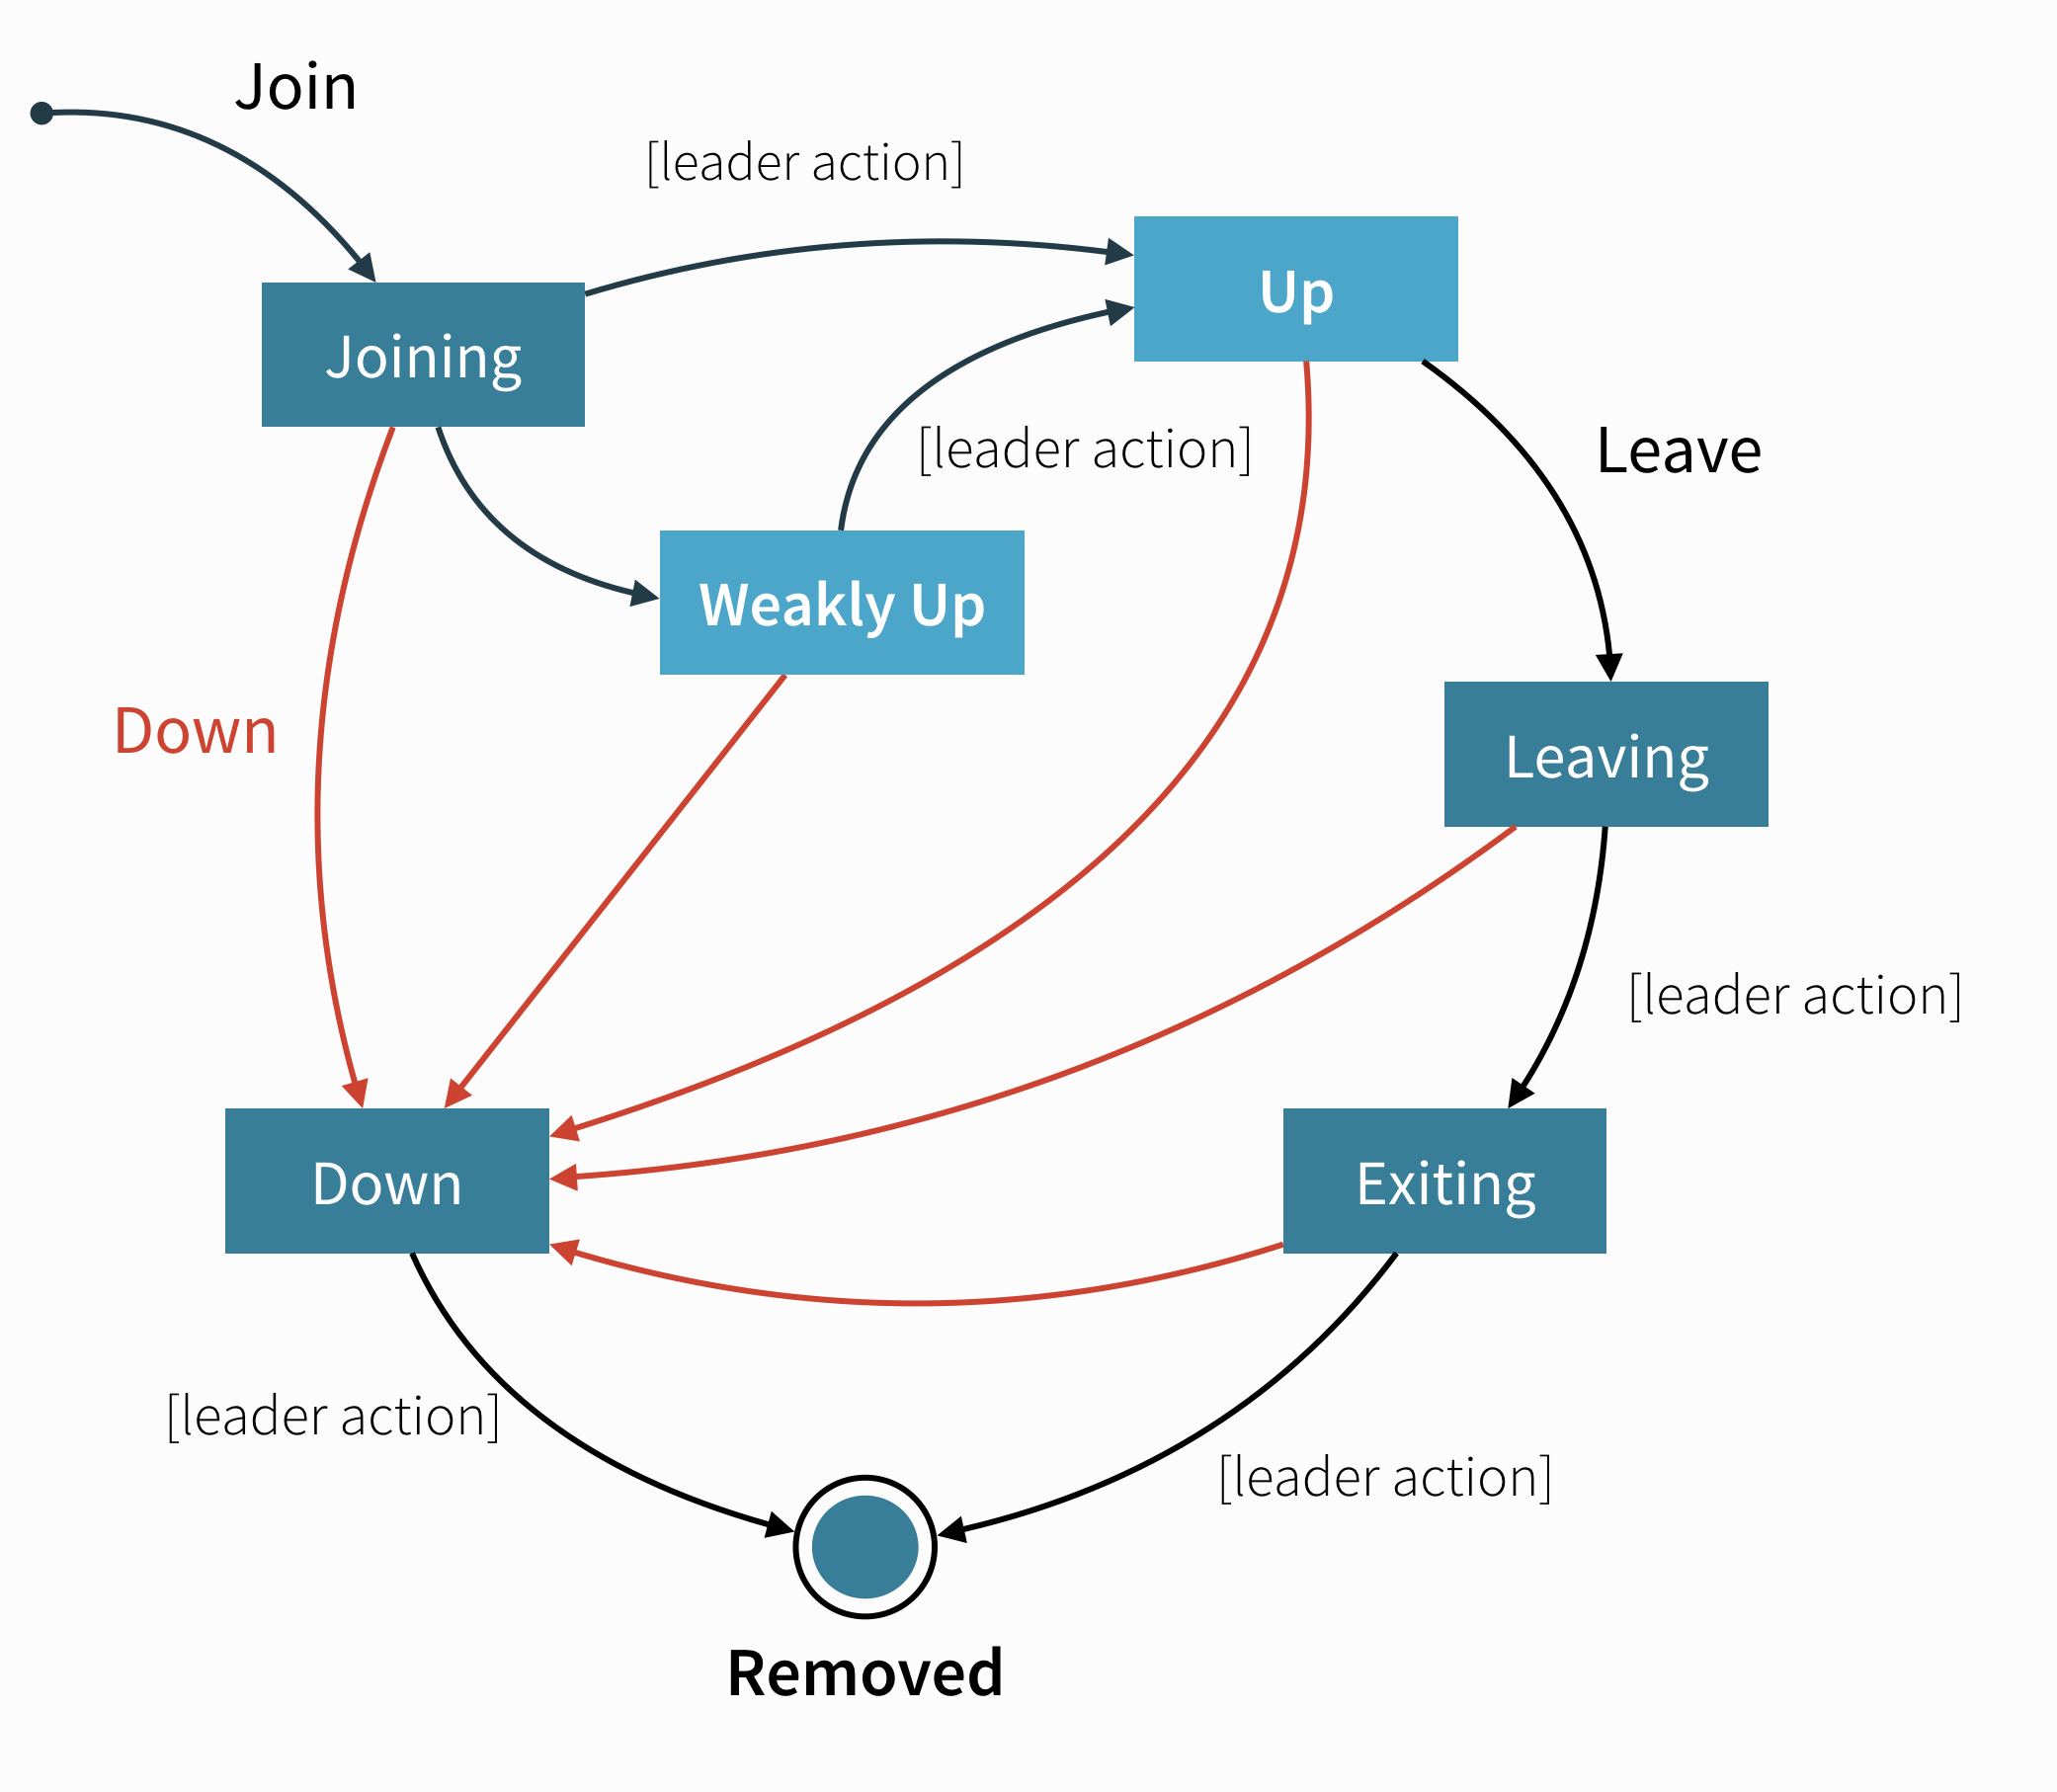
\includegraphics[width=0.6\textwidth]{img/member-state-diagram.png}
	\end{figure}
\end{frame}
\begin{frame}[c, fragile]{Akka Cluster facilities}
\begin{itemize}
	\item \bold{Receptionist} \href{https://doc.akka.io/docs/akka/current/typed/actor-discovery.html}{\faLink}. Registered actors will appear in the receptionist of other nodes of the
	cluster.
	\begin{itemize}
		\item The state for the receptionist is propagated via \ttt{distributed-data} support
	\end{itemize}
	\item \bold{Group router} \href{https://doc.akka.io/docs/akka/current/typed/routers.html}{\faLink}. Created for a \ttt{ServiceKey}, uses receptionist to discover actors, and
	routes messages to available actors
	\begin{itemize}
		\item By using the receptionist, this is cluster-aware out-of-the-box
	\end{itemize}
	\item \bold{Distributed data} \href{https://doc.akka.io/docs/akka/current/typed/distributed-data.html}{\faLink}. The \ttt{\textbf{DistributedData}} extension provides a cluster-wide
	\textbf{key-value} store where values are CRDTs
	\begin{itemize}
		\item Local updates + replication via gossip + conflict-resolution via monotonic merge function
		\item Data types include counters, sets, maps, registers
		\item Read/write access via \ttt{DistributedData(ctx.system).\textbf{replicator}}
	\end{itemize}
	\item Cluster singleton \href{https://doc.akka.io/docs/akka/current/typed/cluster-singleton.html}{\faLink}. Support for managing one singleton actor in the cluster
	\item[] \begin{tcolorbox}[left=0pt, top=0pt, bottom=0pt]
		\begin{minted}{scala}
ClusterSingleton(system).init(SingletonActor(someBehavior()), "MySingleton")
\end{minted}
\end{tcolorbox}
	\item Cluster sharding \href{https://doc.akka.io/docs/akka/current/typed/cluster-sharding-concepts.html}{\faLink} \href{https://doc.akka.io/docs/akka/current/typed/cluster-sharding.html}{\faLink} \href{https://github.com/akka/akka-samples/tree/2.6/akka-sample-sharding-scala}{\faLink}. Distributed and interact with actors based on their logical ID.
 \begin{itemize}
	\item A \bold{Shard} is a group of \bold{entities} managed together.
 	\item Each cluster node has a \bold{ShardRegion} actor that extracts the entity and shard IDs from incoming messages
 	\item A singleton \bold{ShardCoordinator} decides which \ttt{ShardRegion} shall own what \ttt{Shards}; the
 state of shard locations is shared via \ttt{distributed-data}
 \end{itemize}
\end{itemize}
\end{frame}
\begin{frame}[c]{Acknowledgement}
	The material and the slides are derived from Roberto Casadei works \href{https://www.slideshare.net/RobertoCasadei/akka-actors-an-introduction}{\faLink}
\end{frame}
%===============================================================================
\section*{}
%===

%%%%%%%%%%%%%%%%%%%%%%%%%%%%%%%%%%%%%%%%%%%%%%%%%%%%%%%%%%%%%%%%%%%%%%%%%%%%%%%%
\end{document}
%%%%%%%%%%%%%%%%%%%%%%%%%%%%%%%%%%%%%%%%%%%%%%%%%%%%%%%%%%%%%%%%%%%%%%%%%%%%%%%%
